\documentclass[letterpaper,12pt]{article} 
\usepackage[utf8]{inputenc} 
\usepackage[shortlabels]{enumitem}
\usepackage[spanish,mexico]{babel} 
\usepackage{amsmath,amssymb,amsfonts,latexsym,cancel}
\usepackage{hyperref}
\usepackage{wrapfig}
\usepackage[rflt]{floatflt}
\usepackage[pdftex]{graphicx}
\usepackage{fancyhdr} 
\usepackage{float}
\usepackage{longtable,multirow,booktabs}
\usepackage{cite}
\usepackage[square,numbers]{natbib}
\usepackage{multicol}
\usepackage{caption}
\usepackage[]{sidecap}
\usepackage{adjustbox}
\usepackage{parskip}
\usepackage{tikz}
\usepackage{lipsum}
\usepackage{microtype}
\captionsetup[table]{name=Tabel}
\captionsetup[figure]{name=Gambar}
\usepackage{tabulary}
\usepackage{minted}
\usepackage{fancyhdr}
\usepackage{placeins}
\usepackage{graphicx}
\usepackage[all]{xy}
\usepackage{tikz}
\usepackage{verbatim}
\usepackage[top=3cm,bottom=2.5cm]{geometry}
\hypersetup{
    colorlinks,
    linkcolor={red!50!black},
    citecolor={blue!50!black},
    urlcolor={blue!80!black}
}
\usepackage{subcaption}
\usepackage{psfrag}
\usepackage{tcolorbox}
\usepackage[T1]{fontenc}
\usepackage[scaled]{beramono}
\usepackage{listings}
\usepackage{xcolor}
\definecolor{codegreen}{rgb}{0,0.6,0}
\definecolor{codegray}{rgb}{0.5,0.5,0.5}
\definecolor{codepurple}{rgb}{0.58,0,0.82}
\definecolor{backcolour}{rgb}{0.95,0.95,0.92}
\definecolor{LightGray}{gray}{0.9}
\lstdefinestyle{mystyle}{
	backgroundcolor=\color{backcolour},   
	commentstyle=\color{green},
	keywordstyle=\color{codegreen},
	numberstyle=\tiny\color{codegray},
	stringstyle=\color{codepurple},
	basicstyle=\ttfamily\footnotesize,
	breakatwhitespace=false,         
	breaklines=true,                 
	captionpos=b,                    
	keepspaces=true,                 
	numbers=left,                    
	numbersep=5pt,                  
	showspaces=false,                
	showstringspaces=false,
	showtabs=false,                  
	tabsize=2
}
\lstset{style=mystyle}
\renewcommand{\lstlistingname}{Kode}


\thispagestyle{empty}

\begin{figure}[ht]
\minipage{0.7\textwidth}

\includegraphics[width=5cm]{Imagenes/R.jpg}
\label{escudoUV}
		   \endminipage
		   \minipage{\textwidth}
				
\includegraphics[width=5cm]{Imagenes/OIP.jpg}
				\label{EscudoUV}
			\endminipage
		\end{figure}
		
		\vspace{0.1cm}
		
		\begin{center}
		    {\scshape\LARGE \textbf{Universidad Veracruzana} \par}
			{\scshape\Large Facultad de Negocios y Tecnología\par}
			{\scshape\large Ingeniería de Software \par}
            \vspace{0.75cm}
             {\Large \textbf{\myMateria}}

			% Restauramos el interlineado:
			\begin{center}
			
			
			{\Large 402-ISW\myGrupo}
			\vspace{0.75cm}
				
			{\LARGE\bfseries \MyReport\\Paradigmas de Software \myUnidad\par}
            \vspace{0.75cm}
            
		{\scshape\Large 17 de Marzo, 2022 \myDate\par}	
        \vspace{0.75cm}
	    \LARGE	{ \textbf{Centeno Tellez Adolfo}}\\
        \large		{ \myTeacher}
        
		\vspace{0.5cm}	
		
		\LARGE	{ \textbf{Conde Marín Irving Rafael}}
        
        \normalsize	 {\myName}

				\vspace{1.25cm}
				\vspace{0.9cm}
				
			\end{center}
	
		\end{center}
\newpage

\newcommand{\student}{\textbf{Conde Marín Irving Rafael)}}
\newcommand{\course}{\textbf{Paradigmas de Programación)}}
\newcommand{\fecha}{\textbf{17/03/22}}

%%%%%%%%%%%%%%%%%%% using theorem style %%%%%%%%%%%%%%%%%%%%
\newtheorem{thm}{Theorem}
\newtheorem{lem}[thm]{Lemma}
\newtheorem{defn}[thm]{Definition}
\newtheorem{exa}[thm]{Example}
\newtheorem{rem}[thm]{Remark}
\newtheorem{coro}[thm]{Corollary}
\newtheorem{quest}{Question}[section]

\usepackage{lipsum}%% a garbage package you don't need except to create examples.
\usepackage{fancyhdr}
\pagestyle{fancy}
\rhead{ \thepage}
\renewcommand{\headrulewidth}{0.4pt}
\renewcommand{\footrulewidth}{0.4pt}


\newcommand{\N}{\mathbb{N}}
\newcommand{\Z}{\mathbb{Z}}
\newcommand{\Q}{\mathbb{Q}}
\newcommand{\R}{\mathbb{R}}
\newcommand{\C}{\mathbb{C}}
\setlength\headheight{14pt}

\begin{document}
\thispagestyle{empty}
\begin{center}
	
\includegraphics[scale = 0.1]{Imagenes/R.jpg}
\end{center}
\noindent
\rule{17cm}{0.2cm}\\[0.3cm]
Estudiante: \student \hfill Fecha: \fecha\\[0.1cm]
Asignatura: \course \hfill Tema: Hopfield\\
\rule{17cm}{0.05cm}
\vspace{0.1cm}


{\scshape\LARGE \textbf{Introducción} \par}

\section{¿Qué es una red neuronal}

    El término red neuronal se aplica a una familia de modelos relacionada de manera aproximada que se caracteriza por un gran espacio de parámetro y una estructura flexible y que proviene de los estudios sobre el funcionamiento del cerebro. Conforme fue creciendo la familia, se diseñó la mayoría de los nuevos modelos para aplicaciones no biológicas, aunque gran parte de la terminología asociada refleja su origen.

    Las definiciones específicas de redes neuronales son tan variadas como los campos en que se utilizan. Aunque no hay una sola definición que contemple toda la familia de modelos, tenga en cuenta la siguiente descripción por ahora :

    Una red neuronal es un procesador distribuido en paralelo de forma masiva con una propensión natural a almacenar conocimiento experimental y convertirlo en disponible para su uso. Asemeja al cerebro en dos aspectos:

    El conocimiento se adquiere por la red mediante un proceso de aprendizaje.
    
    Las fuerzas de conexión interneuronal, conocidas como ponderaciones sinápticas, se utilizan para almacenar el conocimiento.
\newpage
\section{¿Dónde se utilizan las redes neuronales?}
Las redes neuronales pueden utilizarse en todas las industrias, desde ingeniería a medicina pasando por finanzas. Además, en el área de marketing, las redes neuronales están aportando un gran valor ya que es una herramienta que permite realizar lo siguiente:\newline

Llevar a cabo predicciones sobre el comportamiento futuro de los compradores\newline
Automatizar actividades simples del marketing\newline
Comprender segmentos de compradores\newline
Realizar un pronóstico de ventas\newline
Creación de contenido\newline
 
Su rendimiento destaca especialmente en el análisis de grandes conjuntos de datos, o Big Data Analytics y en consecuencia, el análisis predictivo.
Así, se puede utilizar para mejorar la toma de decisiones empresarial, aumentando las ventas y los ingresos y reduciendo los costes de producción.\newline

Casos de éxito más conocidos \newline

Recomendador de Youtube \newline
Youtube es la compañía más grande del mundo para compartir, crear y visualizar contenido audiovisual. Las recomendaciones de YouTube son responsables de ayudar a más de mil millones de usuarios a descubrir contenido personalizado. Uno de los mayores retos que tuvieron que afrontar a la hora de crear el algoritmo es la cantidad de datos que son subidos a youtube por segundo. Por lo tanto esta red neuronal tiene que tener la capacidad de ser sensible (responsive) tanto al último contenido subido a la plataforma como a las interacciones del usuario con esta.

Dynamic pricing Amazon\newline
Amazon es el líder indiscutible del comercio electrónico. Es conocido por todos que utiliza precios dinámicos, según un estudio Amazon varía los precios más de 2.5 millones de veces al día. El reto de esta red neuronal es que los precios en la era digital deben fijarse en tiempo real basándose en la oferta y la demanda de un determinado producto durante un limitado periodo de tiempo. Compañías como Wallmart o Uber utilizan estos algoritmos para ofrecer precios más competitivos a sus clientes.

Identificar riesgos en banca\newline
HSBC es una de los bancos que utiliza redes neuronales para transformar la forma de procesar los préstamos e hipotecas. Esta compañía usa este tipo de algoritmos de inteligencia artificial para analizar el comportamiento de antiguos clientes y así poder dar una estimación del riesgo para un cliente nuevo a la hora de adquirir una hipoteca o préstamo.

Personalizar las estrategias de marketing\newline
En los últimos años son varias las compañías que utilizan inteligencia artificial para mejorar sus estrategias de marketing. Las redes neuronales son algoritmos los cuales pueden procesar gran cantidad de datos como: perfiles de compradores, patrones de compra o otros tipo de datos específicos para cada empresa. Este tipo de características hacen que sean los algoritmos perfectos para analizar el mercado y proponer una estrategia de marketing personalizada por cliente. Sephora o Starbucks son dos de las compañías que utilizan este tipo de inteligencia artificial para incrementar sus beneficios.

{\scshape\LARGE \textbf{Desarrollo} \par}

\section{Estructura de las redes neuronales}
    
Aunque las redes neuronales plantean exigencias mínimas sobre los supuestos y la estructura del modelo, resulta útil comprender la arquitectura general de la red. La red de perceptrones multicapa (MLP) o de función de base radial (RBF) es una función de predictores (denominados también entradas o variables independientes) que minimiza el error de predicción de las variables de destino (también denominadas salidas).

Tomemos como ejemplo el conjunto de datos bankloan.sav incluido con el producto, en el que desea poder identificar a los posibles morosos entre un grupo de solicitantes de préstamos. Una red MLP o RBF aplicada a este problema es una función de las mediciones que minimiza el error al pronosticar la posibilidad de mora. La figura siguiente resulta muy útil para ilustrar la forma de esta función.

\begin{center}
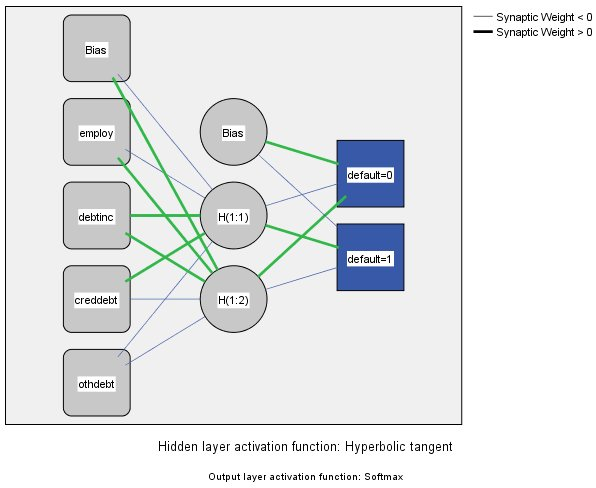
\includegraphics[scale = 0.5]{Imagenes/Estructura_RN.jpg}
\vspace{0.50cm}
\end{center}

Esta estructura se denomina arquitectura feedforward porque las conexiones de la red fluyen unidimensionalmente desde la capa de entrada hasta la capa de salida sin ciclos de retroalimentación. En esta figura:

La capa de entrada contiene los predictores.
La capa oculta contiene nodos (o unidades) no observables. El valor de cada unidad oculta es una función de los predictores; la forma exacta de la función depende, por un lado, del tipo de red y, por otro lado, de especificaciones controlables por el usuario.
La capa de salida contiene las respuestas. Como el historial de moras es una variable categórica con dos categorías, se recodifica como dos variables de indicador. Cada unidad de salida es una función de las entradas ocultas. Nuevamente, la forma exacta de la función depende, por un lado, del tipo de red y, por otro lado, de especificaciones controlables por el usuario.
La red MLP permite una segunda capa oculta; en ese caso, cada unidad de la segunda capa oculta es una función de las unidades de la primera capa oculta, y cada respuesta es una función de las unidades de la segunda capa oculta.

\section{¿Cómo funcionan las redes neuronales?}
Las redes neuronales son un método de cálculo que busca imitar el funcionamiento de las neuronas en un organismo. De esa inspiración extrae un modelo de unidades conectadas entre sí, que generan, transmiten y refuerzan conceptos para llegar a conclusiones determinadas y consolidarlas como conocimiento. 

Las redes neuronales en inteligencia artificial no hacen más que trasladar el funcionamiento biológico al ámbito matemático. Del mismo modo que, al aprender un idioma, nuestro cerebro va averiguando patrones en la gramática, un ordenador procesa unos datos concretos y descubre el parámetro más adecuado para procesarlos.

Los modelos de redes neuronales sirven para que los ordenadores encuentren parámetros y patrones adecuados mediante un entrenamiento. Éste consiste en alimentar el ordenador con datos para que determine criterios válidos de análisis y los aplique.

La unidad de una red neuronal artificial es un procesador elemental llamado neurona que posee la capacidad limitada de calcular, en general, una suma ponderada de sus entradas y luego le aplica una función de activación para obtener una señal que será transmitida a la próxima neurona. Estas neuronas artificiales se agrupan en capas o niveles y poseen un alto grado de conectividad entre ellas, conectividad que es ponderada por los pesos. A través de un algoritmo de aprendizaje supervisado o no supervisado

\newpage

\section{Tipos de redes neuronales}

Clasificación por el número de capas.\newline

Redes neuronales monocapas:\newline 
Generalmente son las más sencillas de hacer, la capa de entrada también podría considarse una capa, pero al no hacer cálculos no se tiene en cuenta a la hora de clasificarse. La capa de entrada se conectan a la capa de neuronas de salida que realizan determinados cálculos.\newline

Redes neuronales multicapas:\newline
Entre las conexiones de entrada y de salida, existen diversas capas de neuronas que hacen de intermediarias, denominadas capas ocultas. Estas capas de neuronas, pueden conectarse entre ellas o no.\newline

Clasificación por los tipos de conexiones.\newline

Redes neuronales no recurrentes:\newline
Se descubrieron en el año 1980, la información de las redes neuronales trabaja en un solo sentido. No existe una realimentación y también carecen de memoria. Este tipo de red neuronal no es tan utilizada. Sin embargo las redes neuronales recurrentes y no recurrentes, también utilizan algoritmos en común como por ejemplo en la fase de entrenamiento.\newline

Redes neuronales recurrentes:\newline
Las neuronas tienen la posibilidad de realizar conexiones realimentación, ya sea entre neuronas de una misma capa o de diferentes capas. La realimentación permite que las redes neuronales recurrentes, tengan memoria. Las redes neuronales recurrentes tienen mayores ventajas en general y suelen ser más potentes, que las redes neuronales no recurrentes.\newline


Clasificación por grado de conexiones.\newline

Redes neuronales totalmente conectadas:\newline
Las capas anteriores y las capas posteriores, están totalmente conectadas. La totalidad de las neuronas están conectadas entre ellas.

Redes parcialmente conectadas: no todas las neuronas están totalmente conectadas entre ellas.\newline

\newpage

\section{Modelo Hopfield}
El modelo de Hopfield
Uno de los principales responsables del desarrollo que ha experimentado la computación neuronal ha sido J. Hopfield, quien construyó un modelo de red con el número suficiente de simplificaciones como para poder extraer información sobre las características relevantes del sistema.

\subsection{Arquitectura}

Este modelo consiste en una red monocapa con N neuronas cuyos valores de salida son binarios : 0/1 ó -1/+1. Las funciones de activación eran del tipo escalón. Se trata, por tanto, de una red discreta con entradas y salidas binarias; posteriormente Hopfield desarrolló una versión contínua con entradas y salidas analógicas utilizando neuronas con funciones de activación de tipo sigmoidal.

Existen conexiones laterales (cada neurona se encuentra conectada a todas las demás) pero no autorrecurrentes (no consigo misma). Los pesos asociados a las conexiones entre pares de neuronas son simétricos (wij = wji)

\begin{center}
    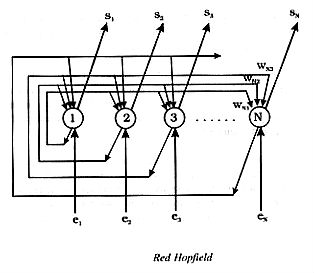
\includegraphics[scale = 0.5]{Imagenes/Arquitectura_Hopfield.jpg}
\end{center}

La versión discreta de esta red fue ideada para trabajar con valores binarios -1 y +1. Por tanto, la función de activación de cada neurona de la red es de tipo escalón:

\begin{center}
    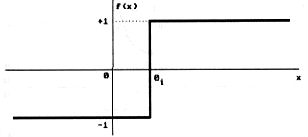
\includegraphics[scale = 0.5]{Imagenes/Arquitectura2_Hopfield.jpg}\newline
f(x) = +1 si x > 0i\newline
f(x) = -1 si x < 0i\newline
f(x) = x si x = 0i\newline
\end{center}

0i es el umbral de disparo de la neurona i, que representa el desplazamiento de la función de transferencia a lo largo del eje de ordenadas (x). En este modelo suele adoptarse un valor proporcional a la suma de los pesos de las conexiones de cad neuorna con el resto:

0i = k SumNj=1 wji

donde :\newline	 
 	Sum es la sumatoria desde j = 1 hasta N\newline
 	k es la constante de proporcionalidad\newline
Si se trabaja con los valores binarios -1 y +1, suele considerarse el valor nulo para 0i. Si los valores son 0 y 1, se toma un valor de 1/2 para k.\newline

\subsection{Funcionamiento}

Se trata de una red autoasociativa. Por tanto, informaciones diferentes (patrones) pueden ser almacenadas en la red, como si de una memoria se tratase, durante la etapa de aprendizaje. Posteriormente, cuando se presenta una entrada a la red, esta evoluciona hasta generar una salida que coincidirá con la que corresponde a esa entrada, o bien la más parecida si la entrada está distorsionada o incompleta.

La información que recibe la red debe haber sido previamente codificada y representada en forma de vector (como una configuración binaria o como un conjunto de valores reales dependiendo de si la red es discreta o contínua) con tantas componentes como neuronas (N) tenga la red. Cada neurona recibe un elemento del vector.

Centrándonos en una sola neurona el funcionamiento sería el siguiente:

\begin{center}
    
1.- Recibe como entrada la salida de cada una de las otras neuronas (por las conexiones laterales). Estos valores de salida, inicialmente coinciden con las entradas del vector, multiplicadas por los pesos de las conexiones correspondientes. La suma de todos estos valores constituirá el valor de entrada neta de la neurona a la que hay que aplicarle la función de transferencia obteniéndose el valor de salida correspondiente. En el instante inicial (t=0) la información de entrada es (e1, e2, ...eN)

\begin{center}
    si(t=0) = ei	 	1 <= i <= N\newline
si(t+1) = f (Sum wij sj(t) - 0i)	 	1 <= i <= N
\end{center}

2.- Este proceso continúa hasta que las salidas de las neuronas se estabilizan, alcanzan la convergencia, durante algunas iteraciones.

\begin{center}
    si(t+1) = si(t)
\end{center}

\end{center}

La red Hopfield continua, con funciones de activación de tipo sigmoidal, ofrece más posibilidades que la discreta ya que permite almacenar patrones formados por valores reales (por ejemplo, imágenes en color o en blanco y negro con diferentes tonalidades de grises).

Otro aspecto importante en el funcionamiento de la red es el instante en que se produce la generación o actualización de las salidas. Si la actualización se realiza de forma simultánea en todas las neuronas el funcionamiento es paralelo o síncrono. Si, por el contrario, las neuronas trabajan de forma secuencial, actualizándose sólo la salida de una neurona en cada iteración, se trata de una red secuencial o asíncrono. En este caso la salida a la que converge la red puede ser diferente en función del orden de la secuencia de activación.

\subsection{Aprendizaje}
El mecanismo de aprendizaje utilizado es de tipo OFF LINE, por lo que existe una etapa de aprendizaje y otra de funcionamiento de la red. También utiliza un aprendizaje no supervisado de tipo hebbiano, de tal forma que el peso de una conexión entre una neurona i y otra j se obtiene mediante el producto de los componentes i-ésimo y j-ésimo del vector que representa la información o patrón que debe almacenar.

Utilizando una notación matricial, para representar los pesos de la red se puede utilizar una matriz de dimensión NxN (recordemos que N es el número de neuronas de la red y por tanto de componentes del vector de entrada). Esta matriz es simétrica (wij = wji) y con la diagonal con valores nulos (wii = 0) al no haber conexiones autorecurrentes.

También tenemos M entradas que la red debe aprender, expresadas igualmente en forma matricial, E1, E2, .., EN

Utilizando esta notación, el aprendizaje consistiría en la creación de la matriz de pesos W a partir de los M vectores de entrada que se enseñan a la red.

\begin{center}
    
W = Sumk=1..N (T(Ek). Ek - I)
\newline 
donde :	Sumk=1..N es la sumatoria para k igual a 1 hasta el número de neuronas, N T(Ek) es la traspuesta de la matriz Ek I es la matriz identidad que anula los pesos de las conexiones autorecurrentes wii
\end{center}

\subsection{Limitaciones}
Existen varios problemas asociados a la red Hopfield. Los dos más importantes se refieren a la cantidad limitada de datos que se pueden almacenar y la necesidad de que estos datos sean ortogonales entre sí.

\begin{center}
    
1.-Número limitado de entradas en la etapa de aprendizaje:
Si se almacenan demasiadas informaciones, durante su funcionamiento la red puede converger a valores de salida diferentes de los aprendidos, con lo que la tarea de asociación entre la información presentada y alguna de las almacenadas se realiza incorrectamente. Esta situación no se produce nunca si el número de informaciones almacenadas es menor o igual que N / (4lnN) siendo N el número de neuronas de la red. Si se permite la posibilidad de un mínimo error en la recuperación de las informaciones almacenadas, suficientemente pequeño para poder identificar dicha infomación, el número de informaciones almacenadas puede ascender por debajo de un 13,8 porciento del número de neuronas de la red.

2.-Ortogonalidad de las informaciones aprendidas:
Si las informaciones almacenadas no son suficientemente diferentes entre sí (no son ortogonales) puede ocurrir que ante una entrada la red no haga una asociación correcta y genere una salida errónea, tal vez la salida correspondiente a otra entrada aprendida que fuese muy parecida.

Lo que se debe conseguir es que las informaciones que se dan a la red durante la etapa de aprendizaje sean ortogonales, lo cual ocurre si se cumple que cada par de patrones de entrada difieren en, al menos N/2 componentes, siendo N el número total de componentes por patrón. Esta condición puede expresarse como:

\begin{center}
Sumi=1..N (ei,k . ei,m) <= 0 para k distinto de m
\end{center}

donde ei,k y ei,m son los valores binarios (+1 o -1) de los componentes i-ésimos de dos vectores (patrones) diferentes (k y m) a almacenar en la red.

Esta condición de ortogonalidad que establece que dados dos patrones de entrada deben diferir en al menos la mitad de sus componentes (distacia Hamming), puede ser relajada, estableciendo una distancia mínima del 30 porciento para que se garantice todavía un funcionamiento aceptable.

\end{center}

\subsection{Aplicaciones}
En cuanto a las aplicaciones más conocidas de este modelo destacan las relacionadas con el reconocimiento de imágenes y de voz, el control de motores y sobre todo la resolución de problemas de optimización. En este último ámbito se ha aplicado para la resolución de ecuaciones y del problema del viajante de comercio, manipulación de grafos, procesado de señales (conversores analógico-digitales) y de imágenes, etc.

A modo de ejemplo y para que sirva como orientación de como se resuelve un problema mediante el modelo de Hopfield, desarrollaremos a continuación el problema del vendedor viajero.

Problema del vendedor viajero (TSP: Travelling Salesman Problem)
Este problema consiste en, dadas N ciudades que tiene que visitar un vendedor, encontrar el camino más corto para, partiendo de una de ellas, visitarlas todas sin pasar más de una vez por cada una y volviendo finalmente a la ciudad de partida.

La complejidad reside en la enorme cantidad de posibles caminos, muchos de ellos de longitud similar. Para N ciudades, el número de rutas alternativas es de N! / (2N). De esta forma, para 5 ciudades existen 12 caminos posibles; para 10 ciudades, el número de rutas es de 181.440.

Vamos a centrarnos en el caso particular de 5 ciudades. En este ejemplo, como hemos dicho anteriormente, existirían 12 rutas cerradas diferentes, cuya longitud dependerá del orden en que se visiten las ciudades.

 	\begin{center}
 	    
        1   2   3   4   5\newline
1   0   20  30  40  35\newline
2   20  0   25  30  15\newline
3   30  25  0   50  35\newline
4   40  30  50  0   20\newline
5   35  15  35  20  0\newline
 	\end{center}


Desarrollo\newline
Este problema puede abordarse utilizando una red Hopfield de N.N neuronas, siendo N el número de ciudades. Aunque la red es de tipo contínuo con valores en el intervalo [0,1], cuando la red se estabiliza, las salidas de las neuronas de la red tendrán valores binarios (1 si la neurona es activa). Cada neurona activa de la red informaría del orden de una ciudad determinada en el recorrido del viajero. Debemos, por tanto, imaginarnos la red como una matriz NxN donde cada fila está asociada a una ciudad, y las columnas con la posición de cada ciudad dentro del recorrido. Así, si la neurona de la fila 2 y columna 3 está activa, nos indicaría que la ciudad número 2 es la tercera en la ruta (w, x, 2, y, z).

El primer paso consiste en encontrar una expresión (bastante compleja) de la función objetivo que se quiere minimizar.

A continuación hay que relacionar esta función objetivo con la función energía de una red Hopfield para obtener una expresión, también bastante compleja, de los pesos de los enlaces de la red.

Por tanto, si se implementa una red contínua de NxN neuronas con unos umbrales y unos pesos con los valores obtenidos anteriormente, se llegará a una situación de estabilidad en la que sólo habrá activa una neurona por cada fila y columna.

Para este ejemplo, la figura representa la situación final de la red cuya longitud total es de 130 km.

\begin{center}
    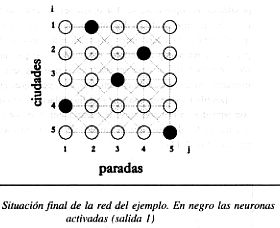
\includegraphics[scale = 0.5]{Imagenes/Ejemplo_Hopfield.jpg}
    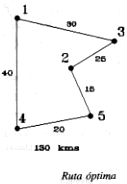
\includegraphics[scale = 0.5]{Imagenes/Ejemplo_Hopfield2.jpg}
    \newline
\end{center}


\section{Ejemplo de Hopfiled}

\begin{tcolorbox}
[colback=red!5!white,colframe=red!75!black,width=15cm ,fonttitle=\bfseries,title=Código  Hopfield Matlab ]

signo suma = [-1,-1,-1,1,-1,-1,-1,-1,-1,-1,1,-1,-1,-1,-1,-1,-1,1,-1,-1,-1,1,1,1,1,1,1,\\1,-1,-1,-1,1,-1,-1,-1,-1,-1,-1,1,-1,-1,-1,-1,-1,-1,1,-1,-1,-1];\\               

signo resta= [-1,-1,-1,-1,-1,-1,-1,-1,-1,-1,-1,-1,-1,-1,-1,-1,-1,-1,-1,-1,-1,1,1,1,1,1\\,1,1,-1,-1,-1,-1,-1,-1,-1,-1,-1,-1,-1,-1,-1,-1,-1,-1,-1,-1,-1,-1,-1];\\

signo multiplicacion = [1,-1,-1,-1,-1,-1,1,-1,1,-1,-1,-1,1,-1,-1,-1,1,-1,1,-1,-1,-1,-1,-1,1,-1,-1,-1,-1,-1,11,1,-1,-1,-1,1,-1,-1,-1,1,-1,1,-1,-1,-1,-1,-1,1];\\

signo division = 
[-1,-1,-1,-1,-1,-1,-1,-1,-1,1,1,1,-1,-1,-1,-1,1,1,1,-1,-1,1,1,1,1,1,1,1,-1,-1,1,1,1,-1,-1,-1,-1,1,1,1,-1,-1,-1,-1,-1,-1,-1,-1,-1];\\

signo igualdad = [-1,-1,-1,-1,-1,-1,-1,-1,-1,-1,-1,-1,-1,-1,1,1,1,1,1,1,1,-1,-1,-1,-1\\,-1,-1,-1,1,1,1,1,1,1,1,-1,-1,-1,-1,-1,-1,-1,-1,-1,-1,-1,-1,-1,-1];\\

signo desigualdad = [-1,-1,-1,-1,-1,-1,-1,-1,-1,-1,-1,-1,1,-1,1,1,1,1,1,1,1,-1,-1,-1,1\\,-1,-1,-1,1,1,1,1,1,1,1,-1,1,-1,-1,-1,-1,-1,-1,-1,-1,-1,-1,-1,-1];\\

signo porcentaje = [-1,-1,-1,-1,-1,-1,1,-1,1,-1,-1,-1,1,-1,1,-1,1,-1,1,-1,-1,-1,1,-1,1\\,-1,-1,-1,-1,-1,1,-1,1,-1,-1,-1,1,-1,1,-1,1,-1,1,-1,-1,-1,1,-1,-1];\\

signo raiz = [-1,-1,-1,-1,-1,-1,-1,-1,-1,-1,-1,1,1,1,-1,-1,-1,-1,1,-1,-1,-1,-1,-1,-1,1\\,-1,-1,1,1,-1,-1,1,-1,-1,-1,-1,1,-1,1,-1,-1,-1,-1,-1,1,1,-1,-1];\\

signo infinito = 
[-1,-1,-1,-1,-1,-1,-1,-1,-1,-1,-1,-1,-1,-1,-1,1,1,-1,-1,1,1,-1,1,-1,1,1,-1,1,-1,1,1,-1,-1,1,1,-1,-1,-1,-1,-1,-1,-1,-1,-1,-1,-1,-1,-1,-1];\\


signo sigma = 
[,1,1,1,1,1,1,1,-1,1,-1,-1,-1,1,-1,-1,-1,1,-1,-1,-1,-1,-1,-1,-1,1,-1,-1,-1,-1,-1,1,-1,-1,-1,-1,-1,1,-1,-1,-1,1,-1,1,1,1,1,1,1,1];

suma = signo suma(:) * signo suma(:)';

resta = signo resta(:) * signo resta(:)';

multiplicacion = signo multiplicacion(:) * signo multiplicacion(:)';

division = signo division(:) * signo division(:)';

igualdad = signo igualdad(:) * signo igualdad(:)';

desigualdad = signo desigualdad(:) * signo desigualdad(:)';

porcentaje = signo porcentaje(:) * signo porcentaje(:)';

raiz = signo raiz(:) * signo raiz(:)';

infinito = signo infinito(:) * signo infinito(:)';

sigma = signo sigma(:) * signo sigma(:)';

\end{tcolorbox}
\newpage
\begin{tcolorbox}
[colback=red!5!white,colframe=red!75!black,width=15cm ,fonttitle=\bfseries,title=Código  Hopfield Matlab ]
w1 = suma+resta+multiplicacion+division+igualdad+desigualdad+porcentaje\\+raiz+infinito+sigma;\\

w = w1 - diag(diag(w1));\\

x = 
[-1,-1,-1,1,-1,-1,-1,-1,-1,-1,1,-1,-1,-1,-1,-1,-1,1,-1,-1,-1,1,1,1,1,1,1,1,-1,-1,-1,1,-1,-1,-1,-1,-1,-1,1,-1,-1,-1,-1,-1,-1,1,-1,-1,-1];\\       
u0 = x;\\
c=1;\\

ulast = x;\\

while(1)\\
  u0 = u0*w;\\
  
  for i=1:1:49\\
    if u0(i)>0\\
      u0(i) = 1;\\
     else\\
      u0(i) = -1;\\
     endif\\
  endfor\\
  
  if (ulast == u0)\\
        
        fprintf('Resultado encontrado: ');\\
        u0\\
        ulast\\
        
      fprintf ('Matrices recorridas hasta hallar el resultado: \%d ', c);\\
     break;  \\
  endif\\

  c = c + 1;\\
  ulast = u0;\\
end\\
\end{tcolorbox}
\newpage
{\scshape\LARGE \textbf{Conclusión} \par}

Las redes neuronales pueden utilizarse en un gran número y variedad de 
aplicaciones, tanto comerciales como militares. \\
Se pueden desarrollar redes neuronales en un periodo de tiempo razonable, con 
la capacidad de realizar tareas concretas mejor que otras tecnologías.\\
 Hay muchos tipos diferentes de redes neuronales; cada uno de los cuales tiene 
una aplicación particular más apropiada. Algunas aplicaciones comerciales son:

    *En la biología\\
    *En las empresas\\
    *En el medio ambiente\\
    *En las finanzas\\
    *En la manufacturación\\
    *En la medicina\\
    *En lo militar

\section{Referencias}

Bibliografía\\

Education, I. C. (17 de 08 de 2020). IBM. Obtenido de https://www.ibm.com/es-es/cloud/learn/neural-networks\\
Figueiras, S. (s.f.). CEUPE. Obtenido de https://www.ceupe.mx/blog/como-funcionan-las-redes-neuronales.html\\\\
Pardo, C. (20 de 07 de 20). Obtenido de enzyme: https://blog.enzymeadvisinggroup.com/redes-neuronales-que-son-y-aplicaciones\\\\
Software, C. (30 de 09 de 2020). Redes Neuronales. Obtenido de https://conectasoftware.com/analytics/redes-neuronales-que-son/

\end{document}
